\documentclass[11pt,a4paper]{article}
\usepackage{ngerman}
\usepackage[ngerman]{babel}
\usepackage[utf8x]{inputenc}
\usepackage[T1]{fontenc}
\usepackage{lmodern}
\usepackage{marvosym}
\usepackage{amsfonts,amsmath,amssymb}
\usepackage{textcomp}
\usepackage{pifont}
\usepackage{ifpdf}
\usepackage[pdftex]{color}
\ifpdf
  \usepackage[pdftex]{graphicx}
\else
  \usepackage[dvips]{graphicx}\fi

\pagestyle{empty}

\usepackage[scale=0.775]{geometry}
\setlength{\parindent}{0pt}
\addtolength{\parskip}{6pt}

\def\firstname{Pascal}
\def\familyname{Bernhard}
\def\FileAuthor{\firstname~\familyname}
\def\FileTitle{\firstname~\familyname's Reformation}
\def\FileSubject{Reformation}
\def\FileKeyWords{\firstname~\familyname, Reformation}

\renewcommand{\ttdefault}{pcr}
\hyphenation{ins-be-son-de-re}
\usepackage{url}
\urlstyle{tt}
\ifpdf
  \usepackage[pdftex,pdfborder=0,breaklinks,baseurl=http://,pdfpagemode=None,pdfstartview=XYZ,pdfstartpage=1]{hyperref}
  \hypersetup{
    pdfauthor   = \FileAuthor,%
    pdftitle    = \FileTitle,%
    pdfsubject  = \FileSubject,%
    pdfkeywords = \FileKeyWords,%
    pdfcreator  = \LaTeX,%
    pdfproducer = \LaTeX}
\else
  \usepackage[dvips]{hyperref}
\fi

\definecolor{firstnamecolor}{RGB}{56,115,179}
\definecolor{familynamecolor}{RGB}{56,115,179}
\hypersetup{pdfborder=0 0 0}

% Gleiche Schriftart für Hyperlinks
\urlstyle{same}


%  Gefrickel um URL-Links vernünftig umzubrechen
\makeatletter
\g@addto@macro\UrlBreaks{
  \do\a\do\b\do\c\do\d\do\e\do\f\do\g\do\h\do\i\do\j
  \do\k\do\l\do\m\do\n\do\o\do\p\do\q\do\r\do\s\do\t
  \do\u\do\v\do\w\do\x\do\y\do\z\do\&\do\1\do\2\do\3
  \do\4\do\5\do\6\do\7\do\8\do\9\do\0}
% \def\do@url@hyp{\do\-}

% Hiermit soll einer übervolle Box verhindert werden -- funktioniert sogar irgendwie
\g@addto@macro\UrlSpecials{\do\/{\mbox{\UrlFont/}\hskip 0pt plus 1pt}}
\makeatother

% Farben werden hier definiert
\definecolor{MidnightBlue}{RGB}{0,103,149}


\begin{document}
\sffamily   % for use with a résumé using sans serif fonts;
%\rmfamily  % for use with a résumé using serif fonts;
\hfill%
\begin{minipage}[t]{.6\textwidth}
\raggedleft%
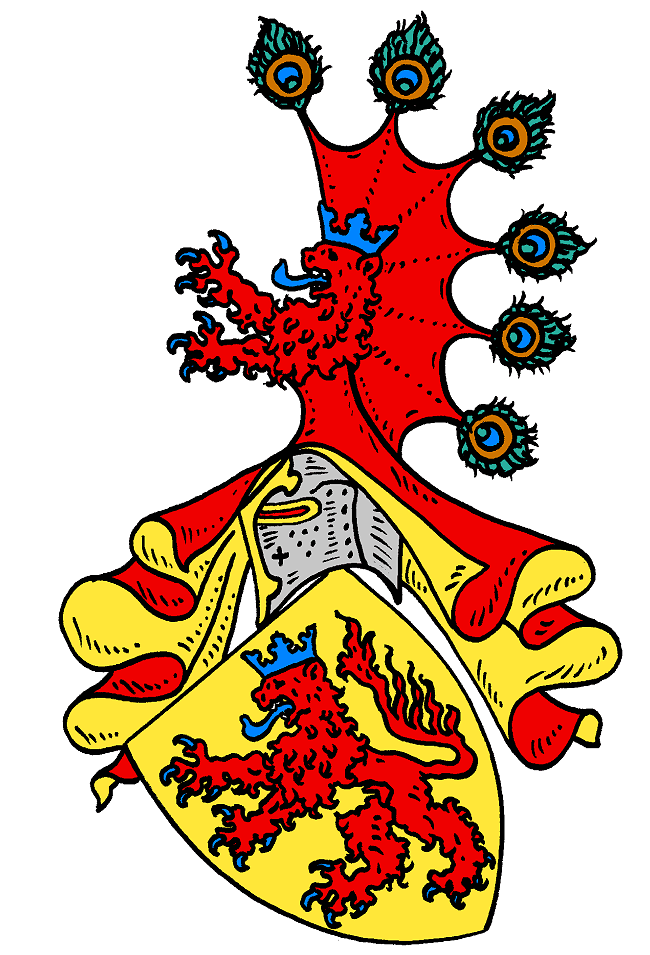
\includegraphics[width=0.55\textwidth]{Habsburg-Stammwappen.png}


%	{\bfseries {\color{firstnamecolor}\firstname}~{\color{familynamecolor}\familyname}}\\[.35ex]
%	\small\itshape%
%	Schwalbacher Straße 7\\
%	12161 Berlin\\[.35ex]
%	\Mobilefone~+49 162 32 39 557 \\
%	\Letter~\href{mailto:pascal.bernhard@rppr.de}{pascal.bernhard@rppr.de}
\end{minipage}\\[0.5em]
%
{\color{firstnamecolor}\rule{\textwidth}{.25ex}}
%
\begin{minipage}[t]{.4\textwidth}
	\raggedright%
	% {\bfseries {\color{firstnamecolor}
	\vspace*{1em}
%	\textbf{Geschichte der Habsburger -- Flaggen} \\
%	 \\[.35ex]
	% }}
	\small%
%	Wolframstraße 89-92\\
%	12105 Berlin
\end{minipage}
%
\hfill
%
\begin{minipage}[t]{.4\textwidth}
	\raggedleft % US style
	\today
	%April 6, 2006 % US informal style
	%05/04/2006 % UK formal style
\end{minipage}\\[2.2em]


{\bfseries \color{familynamecolor}{{\LARGE Die Habsburger Dynastie -- Flaggen}}}\\[0.75em]

\section*{\textsf{Die Geschichte der Habsburger}}

\begin{itemize}
\item Name der Habsburger-Dynastie leitet sich von ihrer Stammburg, der 'Habsburg' im Schweizer Kanton \textsl{Aargau} ab
\item Fürstengeschlecht geht auf den Grafen \textsl{Guntram der Reiche} (\textdied973), der Landbesitz am Oberrhein hatte


\item um 1027 gründete der direkte Nachfahre Radbot (945-1045) mit seiner Ehefrau Ita von Lothringen (995-1035) das Benediktinerkloster \textsl{Muri} im Kanton Aargau

\item als Mittelpunkt der Herrschaft der Fürsten wurde die Habsburg um 1020 errichtet

\item Otto, Graf von Habsburg (\textdied1111) war das erste Familienmitglied, welches sich 'von Habsburg' nannte

\end{itemize}

\subsection*{\textsf{Aufstieg der Habsburger zu einer europäischen Dynastie}}

\begin{itemize}
\item Rudolf IV konnte seinen Herrschaftsraum im späten 13.Jahrhundert systematisch ausbauen\\
\ding{225} Ländereien im Schwarzwald und Herrschaft über die Ost- \& Nordschweiz\\
\ding{225} Krönung zum römisch-deutschen König 1273 (damals gab es noch nicht die Bezeichnung Kaiser) als Rudolf I

\item ab 1278 begann die Herrschaft der Habsburger im heutigen Österreich (Nieder- \& Oberösterreich sowie der Steiermark)\\
\ding{225} Belehnung der Söhne Rudolfs mit den Herzogtümern Österreich und Steiermark

\item Verlust der Schweizer Territorien im 14. und 15.Jahrhundert -- die Habsburg fällt 1415 an die Eidgenossen\\
\ding{225} Machtzentrum der Habsburger verlagert sich nach Osten

\item nachdem er in der \textsl{Goldenen Bulle} nicht als Kurfürst des Heiligen Römischen Reiches berücksichtigt worden war, ließ Rudolf IV eine kaiserliche Urkunde fälschen, die den Österreichischen Stammlanden der Habsburger umfangreiche Rechte (Unteilbarkeit der Länder, eigene Gerichtsbarkeit, automatische Erbfolge, eigene Symbole) zustand und sie als Erzherzogtum deklarierte\\
\ding{225} Urkunde wurde vom damaligen römisch-deutschen Kaiser Friedrich III anerkannt

\item seit der Wahl Albrechts II im Jahre 1438 stellten die Habsburger (mit Ausnahme Kaisers Karls VII 1742-1745) alle Kaiser des Heilgen Römischen Reiches Deutscher Nation

\item durch geschickte Heiratspolitik erwarben die Habsburger Ende des 15. Jahrhunderts die Niederlande, die Freigrafschaft Burgund und darauffolgend die Kronen Böhmens, Spaniens, Kroatien und Ungarns

\item Höhepunkt des Habsburger Reiches mit Karl V, in dessen Weltreich "`die Sonne nie unterging"'

\end{itemize}



\subsection*{\textsf{Die Habsburger in der modernen Neuzeit}}

\begin{itemize}
\item nach dem Tod Karls V

	\begin{enumerate}
	\item allgemeingültige Währung
	\item einheitliches Rechtssystem
	\item (phasenweise) Religionsvielfalt (von den Christenverfolgungen abgesehen)
	\item friedliche Grenzen -- keine Bedrohung von Außen
	\item gemeinsame Sprache
	\item erstrebenswerte Zivilisation
	\end{enumerate}

\item das Römische Reiche hatte einen erheblichen Anteil an der Formierung des politischen und kulturellen Europas in Mittelalter und Neuzeit


	\begin{itemize}
	\item Ausbreitung des Christentums
	\item Etablierung einer Staatsreligion
	\item Latein als Sprache und Mittel zur Bewahrung der Kultur wurde ins Mittelalter übertragen
	\item Latein war bis in die Moderne das einende Element der Europäischen Elite und Kultur
	\end{itemize}

\item römisches Recht bildet Grundlage der Entwicklung moderner europäischer Rechtssysteme

	\begin{itemize}
	\item aus Recht wurde Gesetz
	\ding{225} ohne Gesetz gab es kein Recht (\textsl{sine lege nulla poena})
	\item Recht war niedergeschrieben und nicht willkürlich durch Könige oder Priester ausgeteilt
	\item römisches Recht war auf Lebenspraxis der Bürger und Bedürfnisse nach Gerechtigkeit ausgerichtet
	\end{itemize}

\item durch den Aufstieg der katholischen Kirche trat das kanonische Recht zunehmend gleichberechtigt an die Seite des römischen Rechts

\item in Frankreich, Deutschland und England wurde das auf römischem Rechts basierende System durch Gewohnheitsrecht ergänzt

\item im Zuge der Aufklärung und dem Aufkommen der Idee von Menschenrechten gewann das System logischer Schlussfolgerungen und auf Vernunft basierender Gesetze erneut an Bedeutung



\section*{\textsf{Flaggen der Österreichs, Deutschlands und der Schweiz}}

\subsection*{Schweizer Flagge}


\subsection*{Flagge Österreichs}


\subsection*{Deutsche Flagge}







\end{itemize}


\end{document}